
\section{Results}
\label{outflows:sec:results}

\subsection{Simplified Examples}
\label{outflows:sec:simplified-example}

We begin by comparing the fiducial model from Chapter~\ref{migration} with a
simplified model in which~$\eta = 0$ to highlight generic differences between
models with and without mass loading.
In Chapter~\ref{migration}, the strength of mass loading increases
exponentially with radius according to
\begin{equation}
\eta = \frac{\ycc{O}}{Z_{\text{O},\odot}}
e^{-\grad{O} (\ln 10) (R - R_\odot)} + r - 1.
\end{equation}
Under this parameterization, the equilibrium abundance~$Z_\text{O}$ scales with
radius according to the specified gradient~\grad{O}.
In the case of~$\eta = 0$, the stellar gradient instead arises out of a handful
of effects, including less efficient star formation (i.e., higher~$\tau_\star$)
and a more extended SFH (i.e., high~$\timescale{sfh}$) with increasing radius.
\par
We calibrate a model with~$\eta = 0$ everywhere such that the mode of the MDF
scales with radius according to the gradient we measured
in~\S~\ref{outflows:sec:empirical:gradients}.
The distribution in~$Z$ for some element can be expressed as
\begin{equation}
\frac{dN}{d \ln Z} = Z \frac{dN / dt}{dZ / dt}
\propto \frac{\dot{M}_\star}{(\dot{Z} / Z)}.
\end{equation}
By differentiating the above expression and making a handful of additional
chain rule substitutions, it is straightforward to show that
\begin{equation}
\frac{d^2N}{d \ln Z^2} \propto \dot{M}_\star
\left(\frac{Z}{\dot{Z}}\right)^2
\left(
\frac{\ddot{M}_\star}{\dot{M}_\star} + \frac{\dot{Z}}{Z} -
\frac{\ddot{Z}}{\dot{Z}}
\right).
\end{equation}
Herein lies a portion of our motivation for choosing the mode as our summary
statistic in quantifying abundance gradients.
From the above expression, it is clear that the peak of the MDF is produced
when
\begin{equation}
\frac{\ddot{M}_\star}{\dot{M}_\star} = \frac{\ddot{Z}}{\dot{Z}} -
\frac{\dot{Z}}{Z},
\end{equation}
allowing one to solve for the time at which the peak is produced to determine
its position.
For simple SFHs, such as those in~\S~\ref{outflows:sec:gce:onezone:simple-cases},
the solution is straightforward since one can express~$Z_\text{O}(t)$
analytically.
\par
In the case of a single exponential SFH, differentiating
$\dot{M}_\star \propto e^{-t / \tau_\text{sfh}}$ and
$f_\text{sfh} = 1 - e^{-t / \taupsi{O}}$ (see
Table~\ref{outflows:tab:f-sfh-forms}) and solving for the time~$t_\text{max}$
at which the turnover in the MDF is produced yields
\begin{equation}
t_\text{max} = -\taupsi{O} \ln \left(1 - \frac{\timescale{sfh}}{\taupsi{O}}
\right).
\end{equation}
Computing~\oh~based on~$f_\text{sfh}(t_\text{max})$ indicates that the mode
occurs at
\begin{equation}
\text{mode([O/H])} = \log_{10}
\left(\frac{\ycc{O} \timescale{sfh}}{Z_{\text{O},\odot} \tau_\star}\right).
\end{equation}
\par
In principle, the mode will shift due to changes in both~$\tau_\star$ and
\timescale{sfh}.
Since this is a deliberately simplified example, we do not use the three
component power-law~$\dot{\Sigma}_\star - \Sigma_g$ relationship as in the
$\eta > 0$ comparison case (see discussion below).
We instead take a single power-law, enabling a straightforward solution
for~$\tau_\star$ and therefore~\timescale{sfh} as a function of radius.
By definition,
\begin{equation}
\begin{split}
\Sigma_g \tau_\star^{-1} &\propto \Sigma_g^N
\\
\tau_\star & \propto \Sigma_g^{1 - N}
\\
& \propto e^{(N - 1) R / R_g},
\end{split}
\end{equation}
where~$N$ is the power-law index of the~$\dot{\Sigma}_\star - \Sigma_g$
relation and~$R_g$ is the scale radius of the gas disk.
Combining terms, solving for~$\timescale{sfh}$, and replacing mode([O/H]) with
the desired abundance gradient yields the following relationship between
\timescale{sfh} and~$R$:
\begin{equation}
\tau_\text{sfh} = \tau_{\star,0} \frac{Z_{\text{O},\odot}}{\ycc{O}}
\exp\left[
(N - 1)\frac{R}{R_g} + \grad{O}(\ln 10)(R - R_\odot)
\right],
\label{outflows:eq:tausfh-simplified}
\end{equation}
where~$\tau_{\star,0}$ simply sets the value of~$\tau_\star$ at~$R = 0$,
$Z_{\text{O},\odot}$ is the O abundance in the Sun, and~$R_\odot = 8$ kpc is
the Galactocentric radius of the Sun.
We take~$\grad{O} = -0.06$ kpc$^{-1}$ from our measurements
in~\S~\ref{outflows:sec:empirical:gradients}.
We adopt~$N = 1.5$ based on the global SFRs and surface densities of
low-redshift star forming spirals~\citep{Kennicutt1998}.
Based on the presence of the central molecular zone in the inner few hundred
pc of the Galaxy~\citep[e.g.,][]{Morris1996, Dahmen1998, PiercePrice2000,
Hatchfield2020} and~\citeauthor{Leroy2008}'s~\citeyearpar{Leroy2008}
measurement of~$\tau_\star \approx 2$ Gyr for purely molecular gas, we
attribute this value to~$\tau_{\star,0}$.
We take a scale radius of the gas disk~$R_g = 3$ kpc so that~\timescale{sfh}
increases with radius, as expected from inside-out Galaxy growth
(equation~\ref{outflows:eq:tausfh-simplified} suggests there is a region of
parameter space at high~$R_g$ where the timescale decreases with radius).

\begin{figure*}
\centering
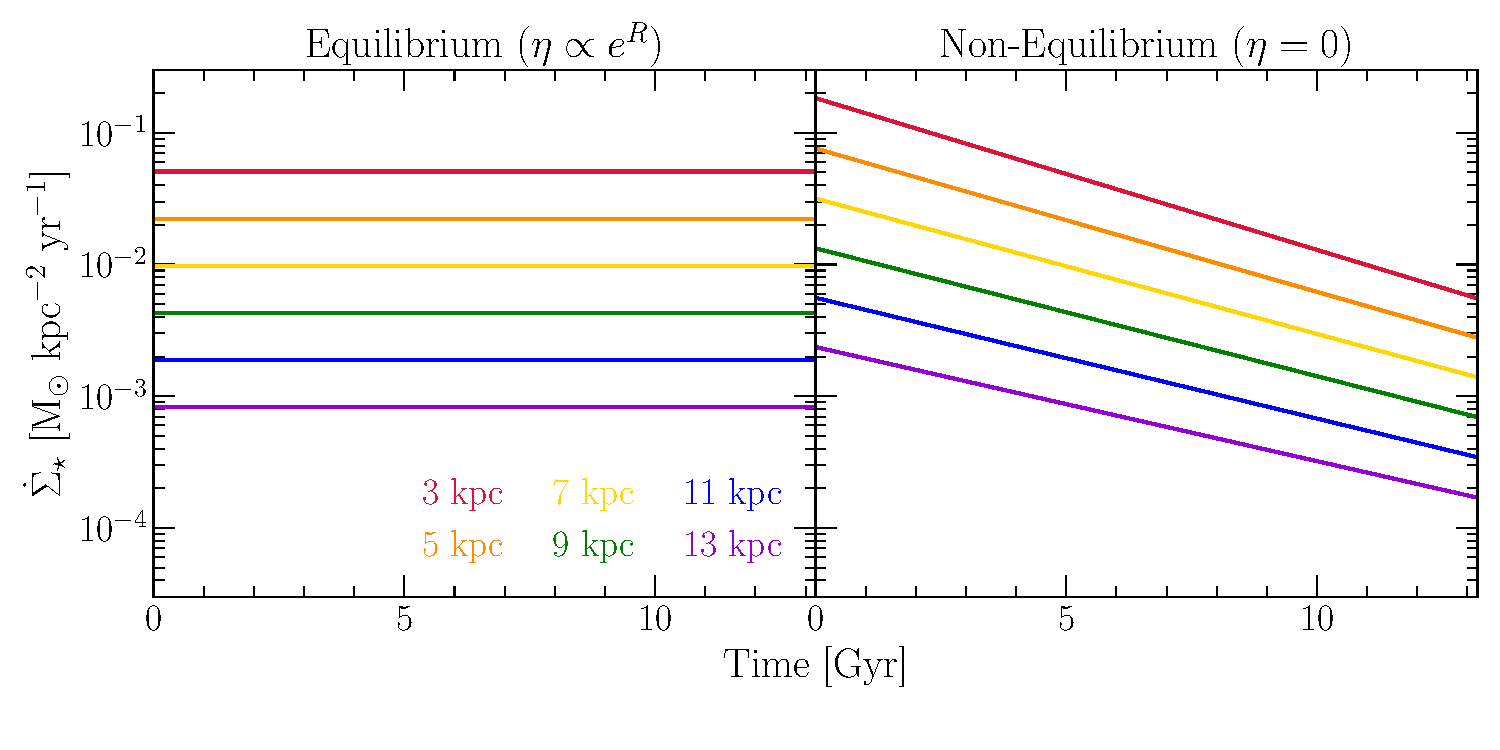
\includegraphics[scale = 0.5]{simplified-examples-sfhs.pdf}
\caption{
SFHs of the~$\eta \propto e^R$ (left) and the~$\eta = 0$ (right) simplified
examples.
Each curve shows the time dependence at a specific radius, color coded
according to the legend.
}
\label{outflows:fig:simplified-examples-sfhs}
\end{figure*}

For a comparison case with~$\eta \neq 0$, we take the model from
Chapter~\ref{migration} with a constant SFH.
In this scenario, it is not the SFH that must be calibrated to the abundance
gradient but~$\eta$ as a function of~$R$.
In Chapter~\ref{migration}, we took an exponential scaling
\begin{equation}
\eta = \frac{\ycc{O}}{Z_{\text{O},\odot}}
e^{-\grad{O}(R - R_\odot)} + r - 1,
\end{equation}
such that the equilibrium abundance varied with radius according to empirical
gradient.

\begin{figure*}
\centering
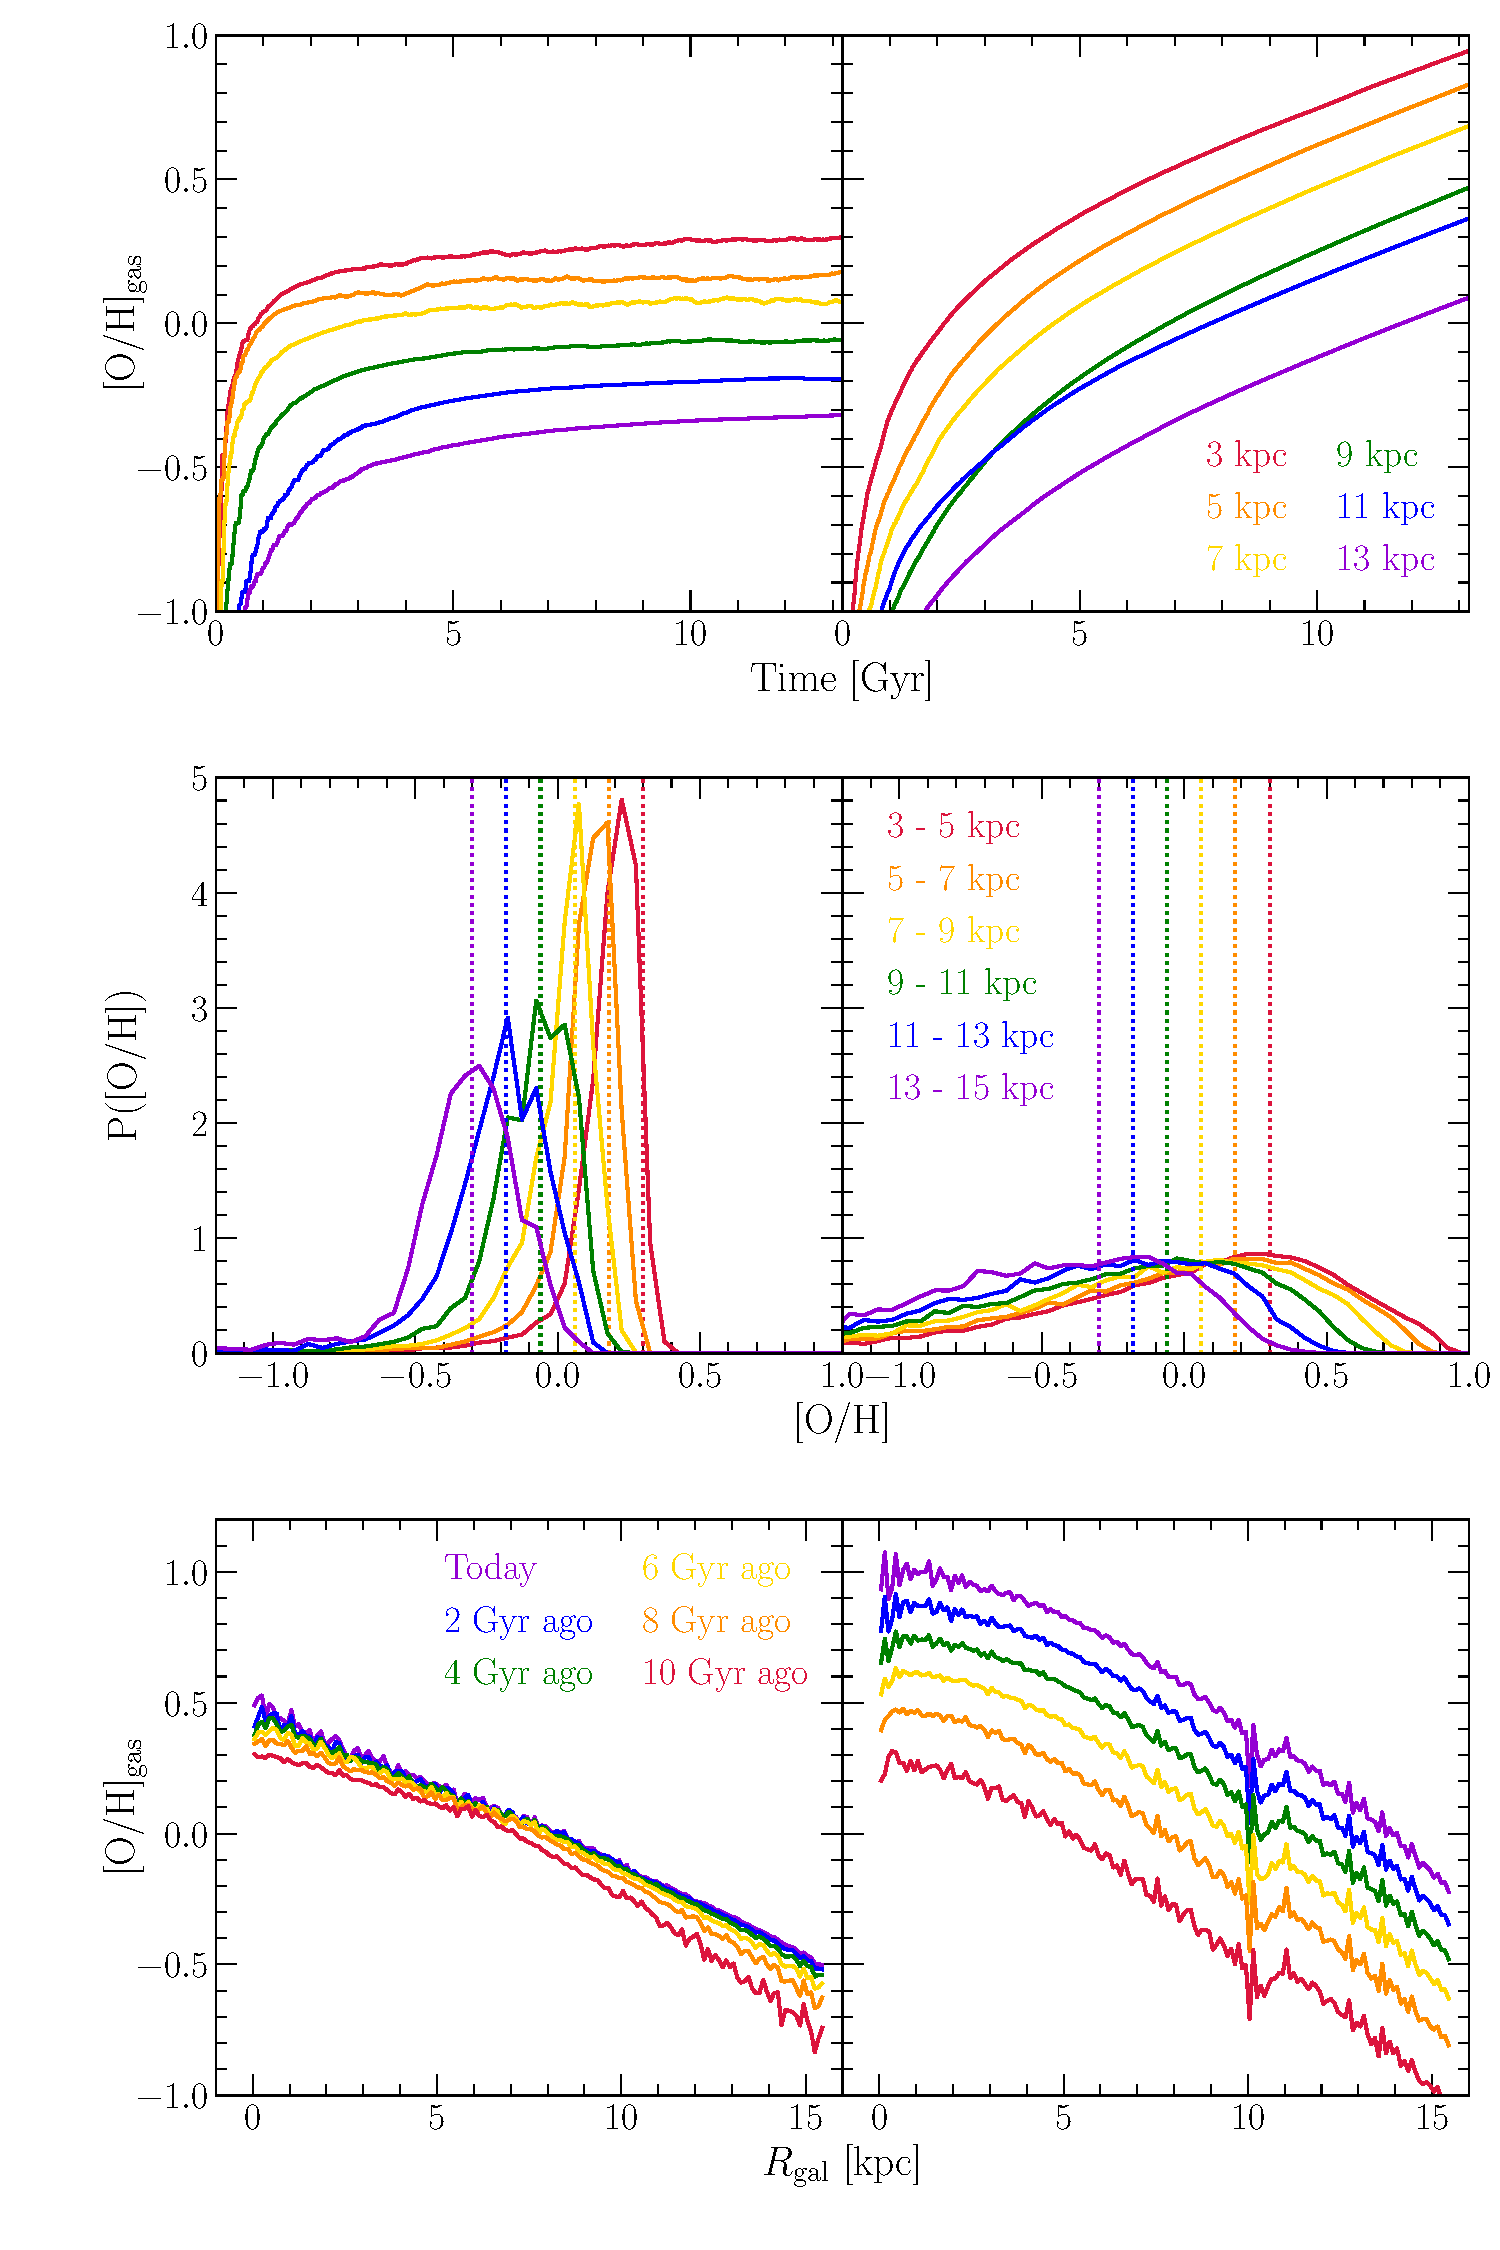
\includegraphics[scale = 0.5]{simplified-examples.pdf}
\caption{
Predicted evolutionary histories of the~$\eta \propto e^R$ (left) and
$\eta = 0$ (right) simplified examples:~\oh~in the ISM at a selection of radii
(top), the distributions in [O/H] in radial bins (middle), and radial
gradients in the gas-phase at snapshots between 2-Gyr intervals (bottom).
Each pair of panels has its own legend identifying the individual curves.
Vertical dotted lines mark the position of the ``target'' gradient with a
slope of~$\grad{O} = -0.06$ kpc$^{-1}$ as measured from our APOGEE sample
in~\S~\ref{outflows:sec:empirical:gradients}.
}
\label{outflows:fig:simplified-examples}
\end{figure*}

Fig.~\ref{outflows:fig:simplified-examples-sfhs} shows the SFHs of these
example models.
The e-folding timescale~\timescale{sfh} varies only marginally with radius
($3 - 5$ Gyr across most radii), indicating that it is mostly the increase
in~$\tau_\star$ driving the abundance gradient.
Fig.~\ref{outflows:fig:simplified-examples} shows the predicted enrichment
histories.
The build up of metals in the ISM is fundamentally different between these two
models.
In the case of~$\eta \propto e^R$,~\oh~increases quickly at early times at all
radii, but reaches the equilibrium abundance after~$\sim$$2 - 3$ Gyr in the
inner disk and~$\sim$$4 - 5$ Gyr in the outer disk.
With~$\eta = 0$, abundances increase up to the present day.
There is an equilibrium abundance in this model, but it is significantly
super-solar, and it simply takes much longer than a Hubble time to reach it.
\par
The differences in metal build up leave a distinct imprint on the stellar
abundance distributions.
In the equilibrium scenario, the distributions are strongly peaked, whereas
they are much broader without mass loading.
In the former, this prediction arises because the ISM forms stars at a similar
abundance for most of the disk lifetime.
In the latter, the peak of the MDF occurs at the ``sweet spot'' calibrated
above, when the rate of star formation becomes too low to populate the upper
end of the MDF.
Due to the ongoing build up of metals without mass loading, the MDF is much
broader.
The ISM simply spends much less time forming stars at one distinct abundance.
\par
The continual build up of metals also leaves distinct features in the gas-phase
gradient at different snapshots in time.
The signature left behind on the radial gradient is an increase in the overall
normalization over time, while the shape remains largely constant.
The equilibrium scenario, by its very nature, instead produces a gradient that
evolves very little between redshift~$z \approx 2$ and the present day.
\par
Lastly, we note an additional reason for choosing the mode as our summary
statistic in quantifying stellar abundance gradients.
The middle row of Fig.~\ref{outflows:fig:simplified-examples} marks the
expected value of~\oh~from our linear fit to the gradient
in~\S~\ref{outflows:sec:empirical:gradients}.
In both models, the MDF peaks extremely close to its intended position.
The only noticeable exception is the~$R = 3 - 5$ kpc bin in the
$\eta \propto e^R$ model, though the difference is~$< 0.1$ dex anyway.
The match between the intended and actual position of the mode is less
obvious in the~$\eta = 0$ model due to the broad nature of the MDFs, so we have
zoomed in on these distributions to verify that they do indeed match well.
At any given radius, stellar migration enhances the metal-rich and metal-poor
tails of the MDF with stars from small~$R$ and large~$R$, respectively.
However, the mode is largely unaffected, indicating that its information
content on the enrichment history in a given Galactic region is relatively
uncontaminated by migration.
The median and especially the mean, on the other hand, are sensitive to the
tails of the MDF.

\subsection{Calibrating to the Gas-Phase Gradient}
\label{outflows:sec:calibrated-model}

We now calibrate a model with~$\eta = 0$ to reproduce the gas-phase gradient at
the present day.
While this observable arises as a consequence of the~$\eta \propto e^R$
specification in Chapter~\ref{migration}, it depends much more strongly on the
detailed SFH without mass loading.
To this end, we take the inside-out SFH (see
equation~\ref{outflows:eq:inside-out-sfh}) and tune~\timescale{rise}
and~\timescale{sfh} such that the present-day ISM abundances line up with
\citeauthor{MendezDelgado2022}'s~\citeyearpar{MendezDelgado2022} measurements
(see Fig.~\ref{outflows:fig:gradxh-gradage} and discussion
in~\S~\ref{outflows:sec:empirical:gradients}).
\par
Drawing on the results of~\S~\ref{outflows:sec:gce:onezone:simple-cases}, the
build up of O in the ISM will proceed according to the appropriate form
of~$f_\text{sfh}$ from Table~\ref{outflows:fig:f-sfh-forms}, modulo the impact
of stellar migration and radial flows.
As a fiducial choice of parameters, we retain~$R_g = 3$ kpc,
$\tau_{\star,0} = 2$ Gyr,~$\eta = 0$,~$\grad{O} = -0.06$ kpc$^{-1}$,~$N = 1.5$,
and~$v_g = 0$ from~\S~\ref{outflows:sec:simplified-example} above.
Given these choices, the only remaining unknowns before the full time evolution
of~$Z_\text{O}(t)$ is known are~\timescale{rise} and~\timescale{sfh}.

\begin{landscape}
\begin{figure*}
\centering
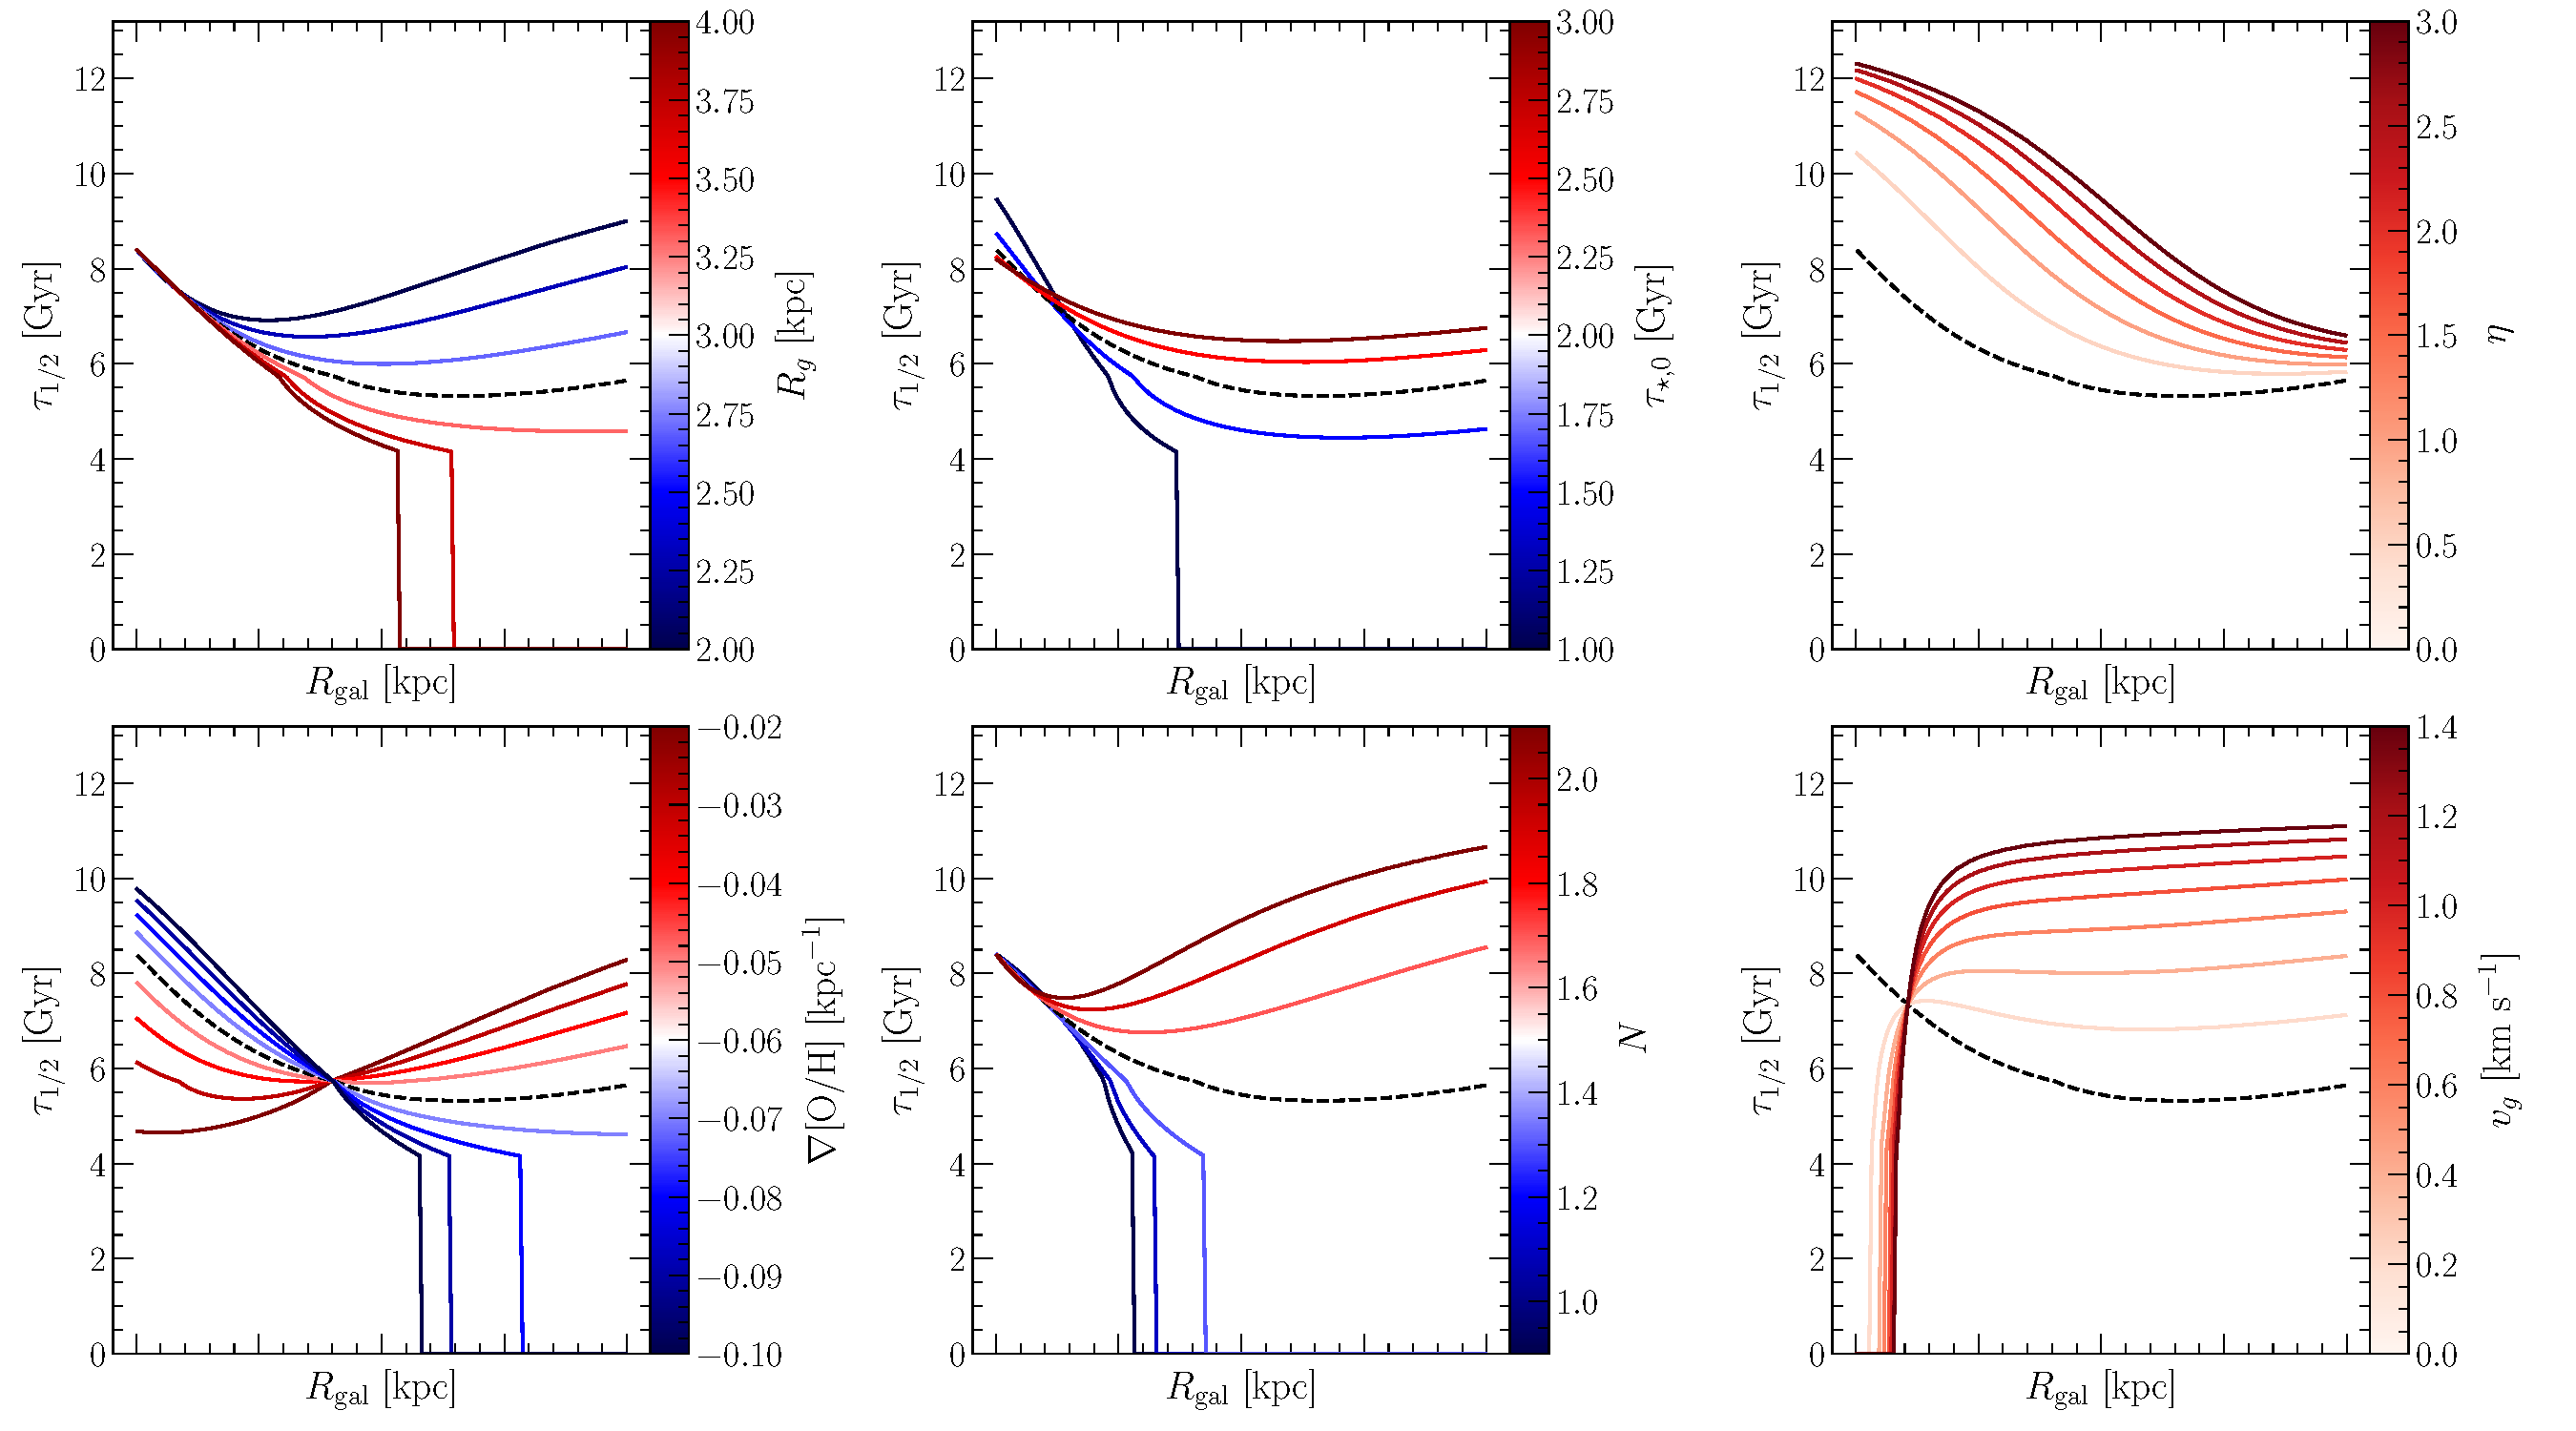
\includegraphics[scale = 0.4]{medage_inputparams.pdf}
\caption{
Median age as a function of radius.
}
\label{outflows:fig:medage-inputparams}
\end{figure*}
\end{landscape}

Following Chapter~\ref{migration}, we initially set the rise timescale
to~$\timescale{rise} = 2$ Gyr.
We then attempt to solve for~\timescale{sfh} via bisection.
If the value exceeds~$\timescale{sfh} = 200$ Gyr (essentially flat
at~$t >> \timescale{rise}$), we then hold it fixed there and solve for the
value of~\timescale{rise}.
If this value also exceeds~$200$ Gyr, then we conclude that there is no
physical solution under the given parameter choice.
We then map~\timescale{rise} and~\timescale{sfh} to the median age of stellar
populations~$\tau_{1/2}$ by integrating over the implied SFH with an assumed
disk lifetime of~$\timescale{disk} = 13.2$ Gyr.
\par
{\color{red} Potentially move this to a discussion section.}
Fig.~\ref{outflows:fig:medage-inputparams} shows the results of applying this
procedure as a function of radius and exploring variations in the individual
parameters.
The sensitivity of the predicted age gradient to the input parameters
underscores a key difference between the~$\eta = 0$ and~$\eta \propto e^R$
scenarios.
Without mass loading and variations thereof with radius, the shape of the SFH
is all there is to vary between Galactic regions.
If the shape of the SFH (i.e., inside-out galaxy growth) is the primary
mechanism behind the radial abundance gradient, then it is directly connected
to the age gradient.
\par







































